\addchap{Appendices}

\begin{appendix}
\renewcommand\thesection{\Alph{section}}

\section{Hyperlink to Deployed Frankenbot\label{appen:deplFrank}}
     \textit{URL to deployed Frankenbot: } \url{https://www.dfki.de/frankenbot/shahid/index.html}

\section{Information for Participants\label{appen:info}}
I am the detective chat bot designed to interrogate you about the armed robbery happened few days back at a spatkauf near Berliner Strasse. I am responsible for its investigation, so I am going to ask you some questions to come up with a decision. It will include, what I have investigated so far. Also you can have general conversation with me like you can ask me to talk about general stuff with you, about corona virus and its stats, to make you laugh, to do gossips, how do I feel, who am I, what do I eat and other related questions about me. You can switch between the topics at any moment as I am designed for parallel handling of the multiple topics. Kindly, chat at least with me until I reach any decision or say you goodbye before you jump to completion of the surveys. Thanks!
\\~\\
Note: If you ever lost where were you and want to reinstate the detective game then just send me a greeting message (hi, hello etc.) and I will restart it for you.

\section{Instructions for Participants\label{appen:instr}}
Just think like you are accused of a robbery and you are sitting in front of a detective and you have to answer his brutal and tricky questions in order to prove your innocence otherwise, you will be declared a culprit. It is a responsibility of a detective to make a decision based on your answers to his questions.
\\~\\
Note: It is the fictional detective chat bot designed only for testing and fun purpose. Have fun while staying safe at home :)

\section{Request for Participants\label{appen:req}}
Once, you are finished having fun with me. Please don't forget to complete following assessments provided as the links below. They will be activated after 1 minute, meanwhile you should get familiar with me by having a small chat with me. I welcome and highly appreciate your prestigious feedback which will help my developer to evaluate me and enhance my abilities for your better experience. Thanks in advance :)

\section{Frankenbot's Dialogue Structure  (frankenbot.json)\label{appen:frankJson}}
    \item \textit{URL to Frankenbot Dialogue Structure: }\url{https://bitbucket.org/nordpolemil/modular-chatbot/src/5ea57ec/frankenbot-framework/bot_def/detective/frankenbot.json?fileviewer=file-view-default}

\section{RASA NLU Training Data Stats\label{appen:traindatastats}}

\subsection{Module 1(detective\_tree.json)\label{appen:detectiveJson}}
\begin{itemize}
    \item intent examples: 115 (6 distinct intents)
	\item Found intents: '\#negation', '\#purchasing', '\#bye', '\#affirm', '\#robbery\_time\_info', '\#greet'
	\item entity examples: 2 (1 distinct entities)
	\item found entities: '@place'
	\item \textit{URL to Training Data for Detective Module: }\url{https://bitbucket.org/nordpolemil/modular-chatbot/src/5ea57ec/frankenbot-framework/bot_def/detective/rasa/detective\_tree.json?fileviewer=file-view-default}
\end{itemize}
	
\subsection{Module 2(general\_tree.json)\label{appen:generalJson}}
\begin{itemize}
    \item intent examples: 205 (9 distinct intents)
	\item Found intents: '\#humor', '\#botFood', '\#gossip', '\#botProfile', '\#psychology', '\#emotion', '\#coronaStats', '\#general\_talk', '\#corona'
	\item entity examples: 41 (1 distinct entities)
	\item found entities: '@feeling'
	\item \textit{URL to Training Data for General Module: }\url{https://bitbucket.org/nordpolemil/modular-chatbot/src/5ea57ec/frankenbot-framework/bot_def/detective/rasa/general\_tree.json?fileviewer=file-view-default}
\end{itemize}
    

\section{RASA Configuration File(config\_spacy.yaml)\label{appen:rasaConf}}
\begin{lstlisting}[language=json, firstnumber=1]
language: "en_core_web_sm"
pipeline:
  - name: "SpacyNLP"
  - name: "WhitespaceTokenizer"
  - name: "SpacyTokenizer"
  - name: "SpacyFeaturizer"
  - name: "SklearnIntentClassifier"
  - name: "CRFEntityExtractor"
  - name: "EntitySynonymMapper"
\end{lstlisting}
\textit{URL to a file: }\url{https://bitbucket.org/nordpolemil/modular-chatbot/src/5ea57ec/frankenbot-framework/bot_def/detective/rasa/config\_spacy.yaml?fileviewer=file-view-default}

\section{Surveys\label{appen:survey}}

\subsection{Frankenbot's Experience Survey\label{appen:expsurvey}}
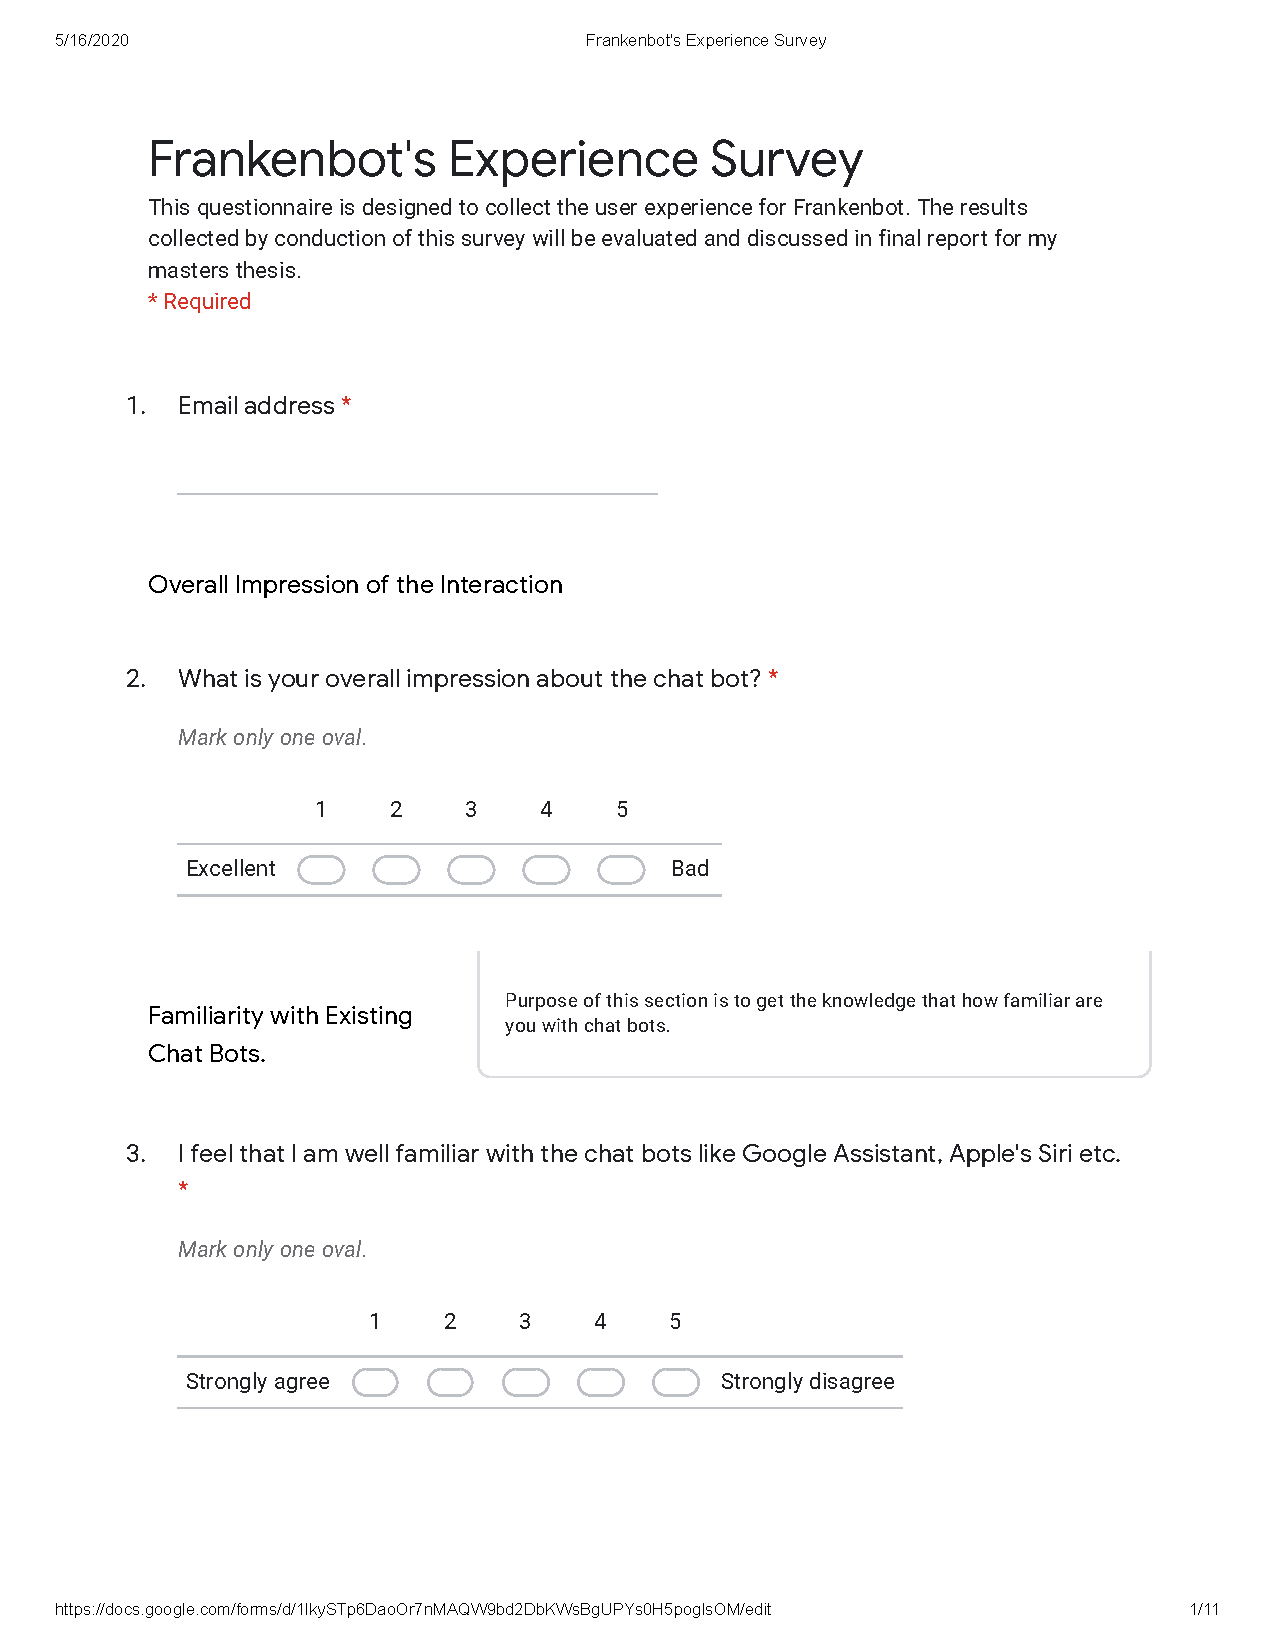
\includepdf[scale=0.9, pages=-]{img/Frankenbot_Experience_Survey.pdf}

\subsection{Frankenbot's Evaluation via AttrakDiff\label{appen:attrsurvey}}
\begin{figure}[!h]
    \centering
    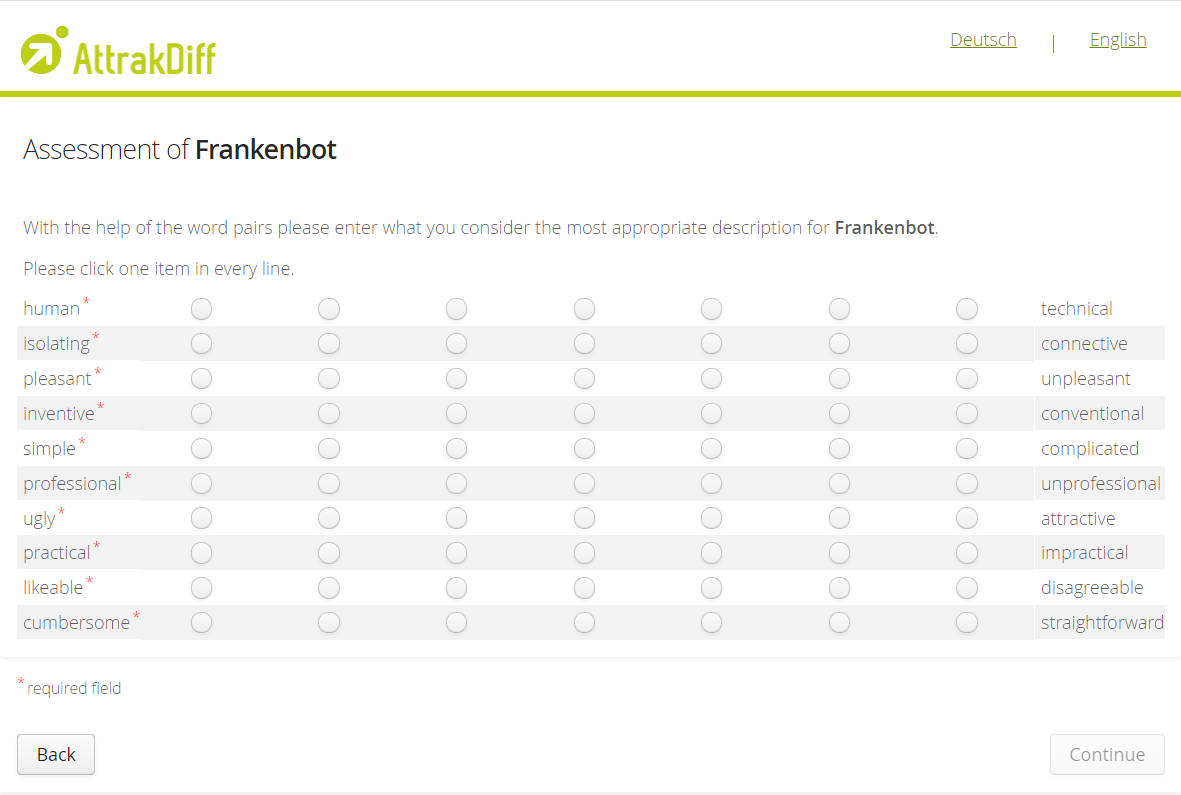
\includegraphics[width=0.9\textwidth]{img/AttrakDiff_Survey_1.PNG}
    \caption{Page 1 \cite{attrakdiff}}
    \label{fig:attr1}
\end{figure}

\begin{figure}[!h]
    \centering
    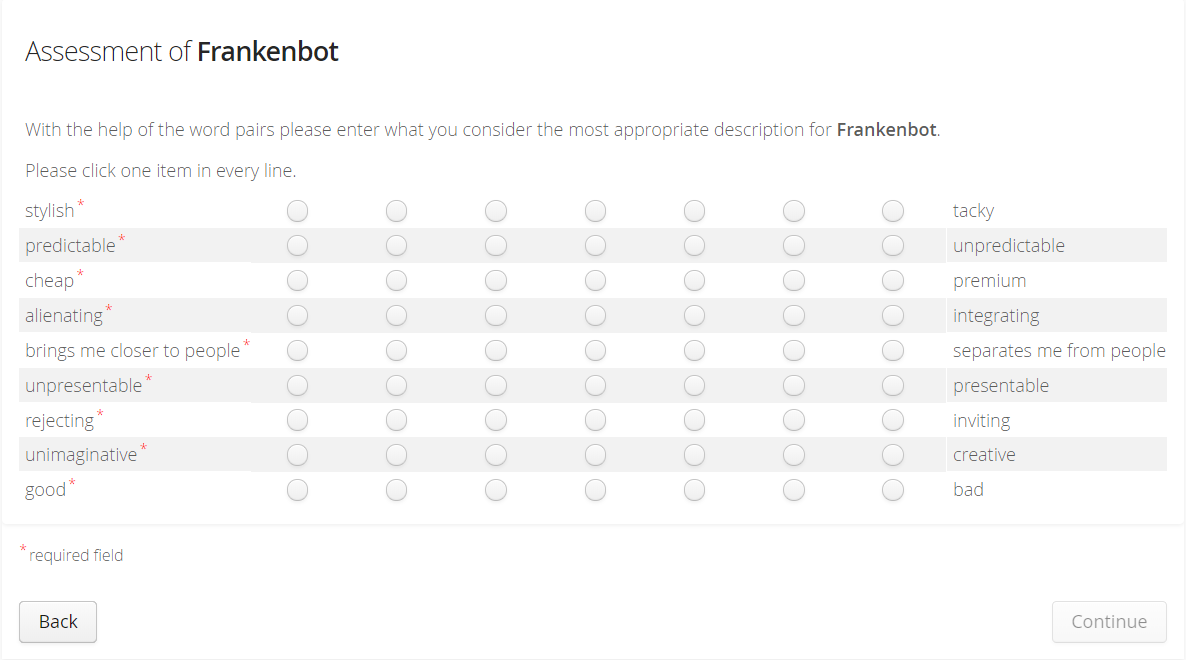
\includegraphics[width=0.9\textwidth]{img/AttrakDiff_Survey_2.PNG}
    \caption{Page 2 \cite{attrakdiff}}
    \label{fig:attr2}
\end{figure}

\begin{figure}[!h]
    \centering
    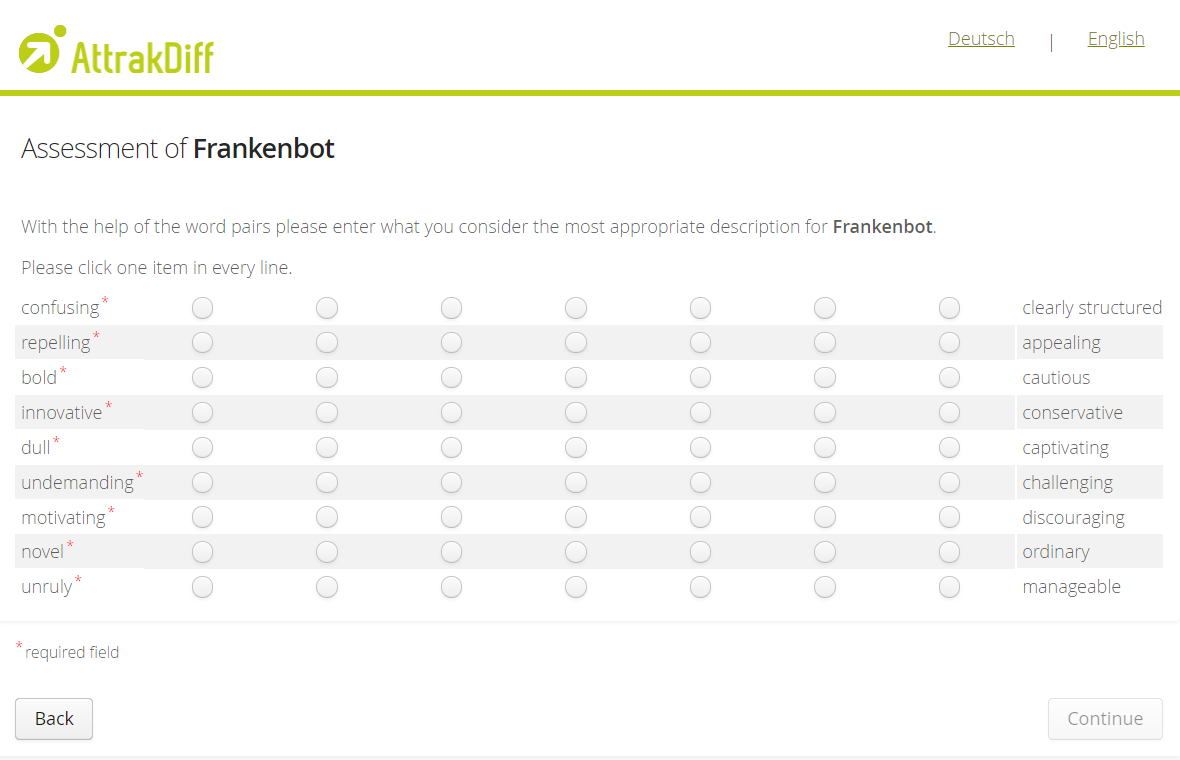
\includegraphics[width=0.9\textwidth]{img/AttrakDiff_Survey_3.PNG}
    \caption{Page 3 \cite{attrakdiff}}
    \label{fig:attr3}
\end{figure}

\begin{figure}[!h]
    \centering
    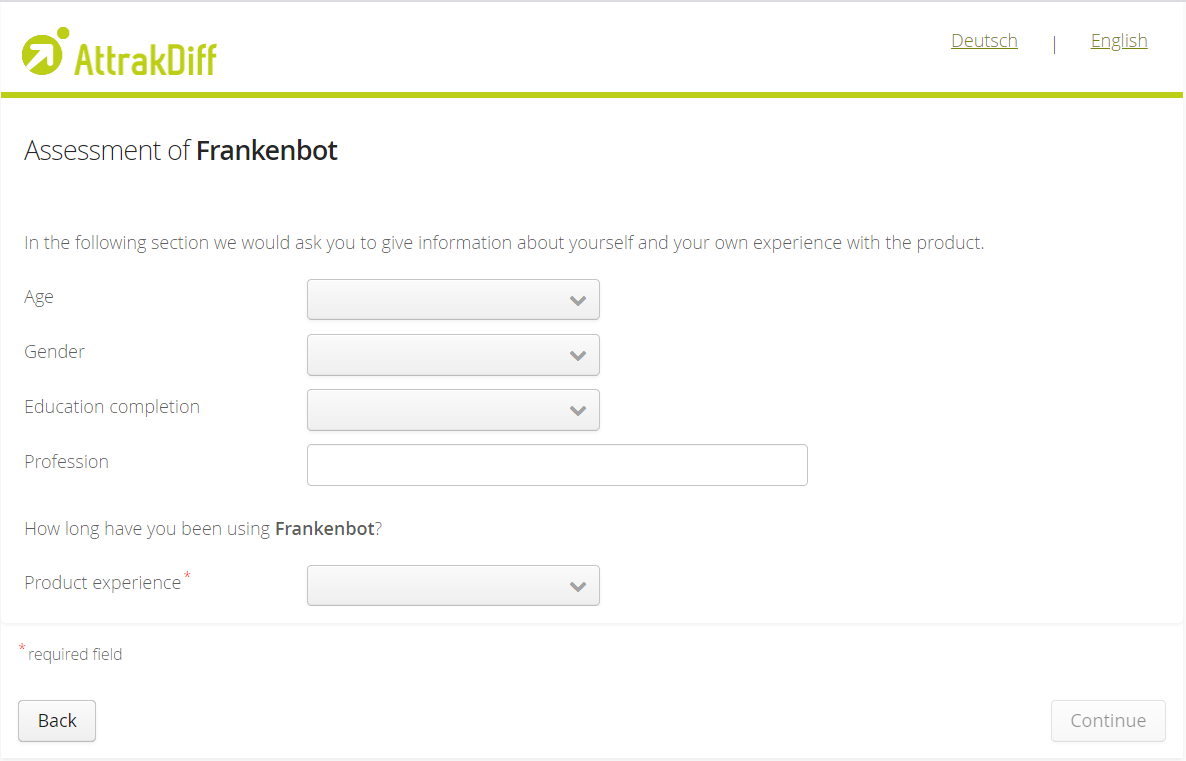
\includegraphics[width=0.9\textwidth]{img/AttrakDiff_Survey_4.PNG}
    \caption{Page 4 \cite{attrakdiff}}
    \label{fig:attr4}
\end{figure}

% \section{Chtabot's Structure File(frankenbot.json)\label{appen:frankJson}}

% \section{Training Data Files\label{appen:trainDF}}
% \subsection{Module 1(detective\_tree.json)\label{appen:detectiveJson}}
% \subsection{Module 2(general\_tree.json)\label{appen:generalJson}}


\end{appendix}

\endinput